\documentclass{article}

\usepackage{graphicx}
\usepackage{subcaption}
\usepackage[margin=1in]{geometry}			%margins
\usepackage{indentfirst}					%indentation
\usepackage{listings}						%code

\setlength{\intextsep}{15pt plus 1.0pt minus 2.0pt}		%figure spacing inside text

\begin{document}

\title{STAT 239 Homework 2}
\author{Tarek Tohme}
\date{April 29th, 2018}
\maketitle

\section{Challenger Disaster}
\paragraph{Question 1}
A logistic model was used to predict the probability of a failure as a function of temperature and pressure. The response is modified to be true if at least one o-ring failed, and false otherwise.

\paragraph{}
logReg1 is the model with only temperature as a predictor, and logReg2 the one with both temperature and pressure. For logReg1 the estimator was -0.2322 � 0.1082, which means for every unit increase in temperature, the response decreases by 0.2322, which means the odds of failure get divided by about 1.25. For logReg 2 the estimate was -0.2415 � 0.1097.

% Figure 1: Telemetry data
\begin{figure}[h]				%placement (here)
	\centering
	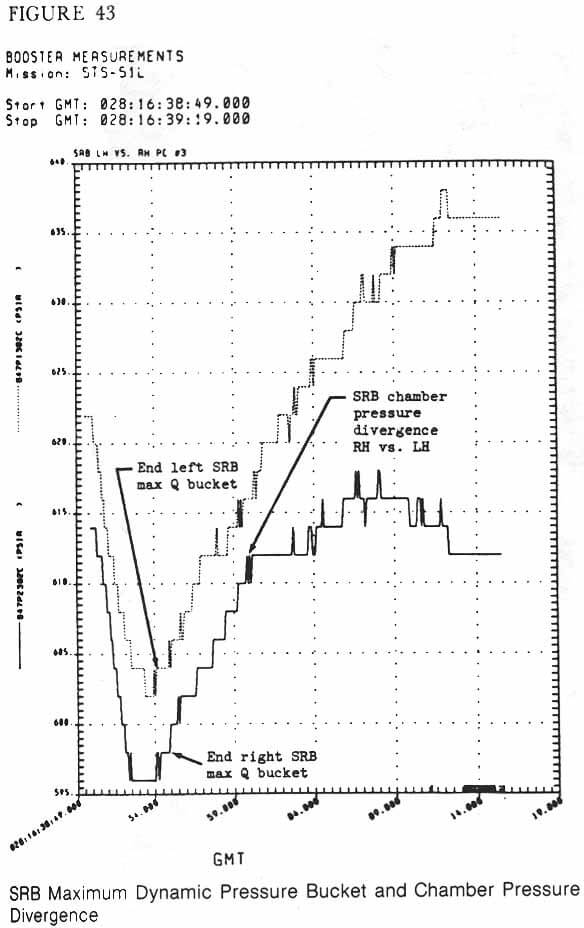
\includegraphics[width=6cm]{Part1_telemetry}
	\caption{Telemetry data from NASA showing internal pressures of both SRBs during the flight. According to NASA telemetry data, pressure was 610 psi at time of o-ring failure. (source: www.spaceflightnow.com)}
\end{figure}

\paragraph{}
There is little difference between both models in terms of deviance and temperature estimates. This shows that pressure doesn't have a strong effect on the model's fit. The responses for some relevant temperatures and pressures are shown in Figure 1: the estimated probability of a failure is 0.999997 according to logReg2, and 0.999609 as predicted by logReg1. According to NASA telemetry data, the internal pressure of the right SRB (the one that got fractured and caused the explosion) was 610 psi just before the pressure started to drop abnormally. However, even with 50 psi as a predictor, the estimated probability is still 0.999357.

\paragraph{Question 2}
The following figures show the predicted probabilities of failure and success for LDA and QDA. 

% Figure 2: LDA
\begin{figure}[h]				%placement (here)
	\centering
	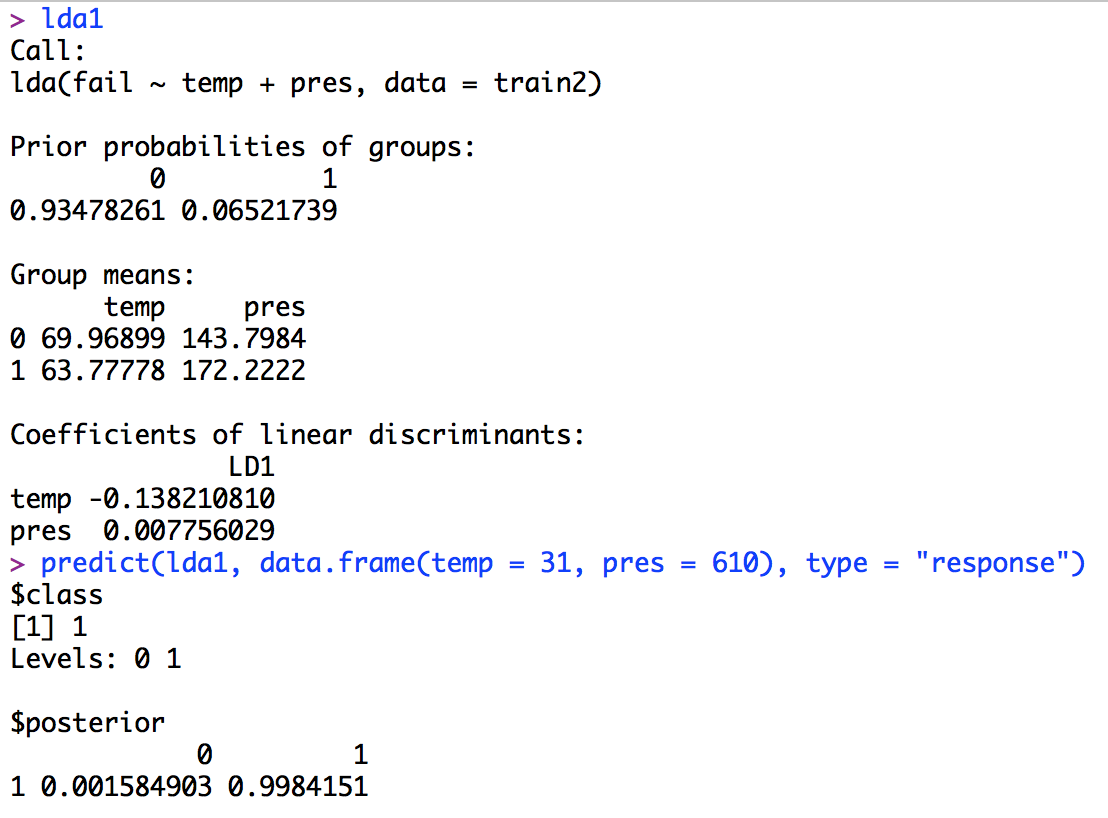
\includegraphics[width=11cm]{Part1_lda}
	\caption{LDA}
\end{figure}

% Figure 3: QDA
\begin{figure}[h]				%placement (here)
	\centering
	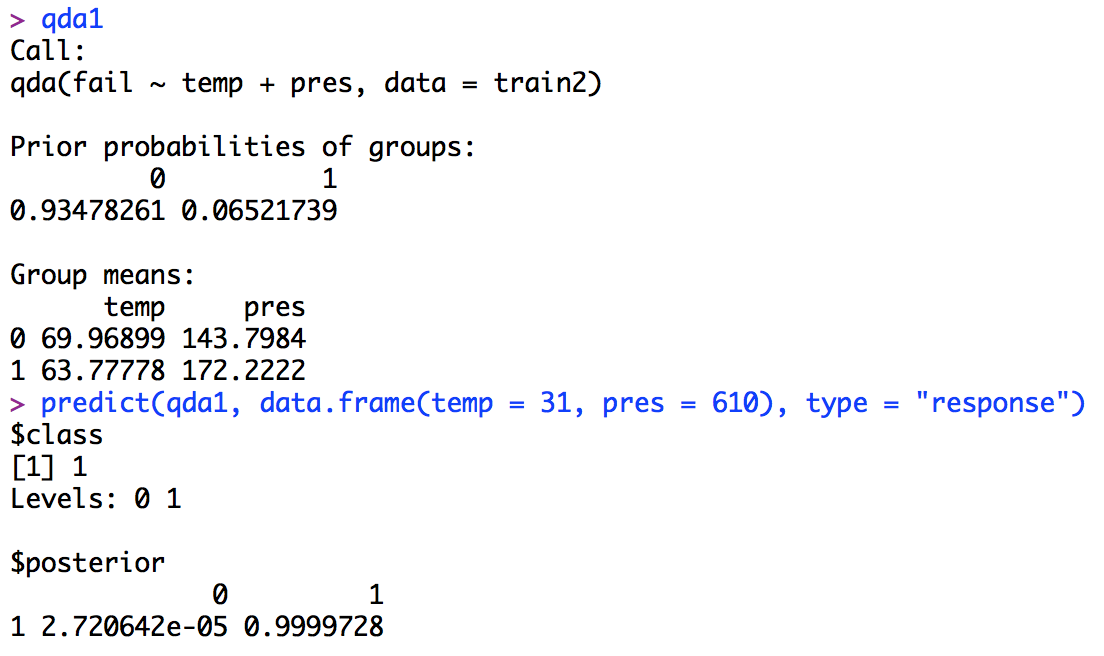
\includegraphics[width=11cm]{Part1_qda}
	\caption{QDA}
\end{figure}

\paragraph{}
According to all three models, the chance of failure given the conditions of the launch were overwhelmingly high.

\section{Titanic Disaster}

\paragraph{Question 1}
Figure 4 below shows four separate tables where each corresponds to a combination of sex and age, and the ratios of surv vs m against class for each table . By visual comparison, the predicted values don't match the prior probabilities very well, except for adult females. Also, in the frequencies plot in Figure [ ], we see that sex and age are noticeably correlated: there is a difference in the way sex affects the frequency of survival when age is varied, holding class fixed. For children, sex doesn't affect survival at all, but for adults it does. The range of survival frequencies for adult males was 0.1 to 0.35 whereas for adult females it was 0.45 to 0.95. Therefore, this model isn't very adequate without at least one interaction parameter.

% Figure 4: priors
\begin{figure}[h]				%placement (here)
	\centering
	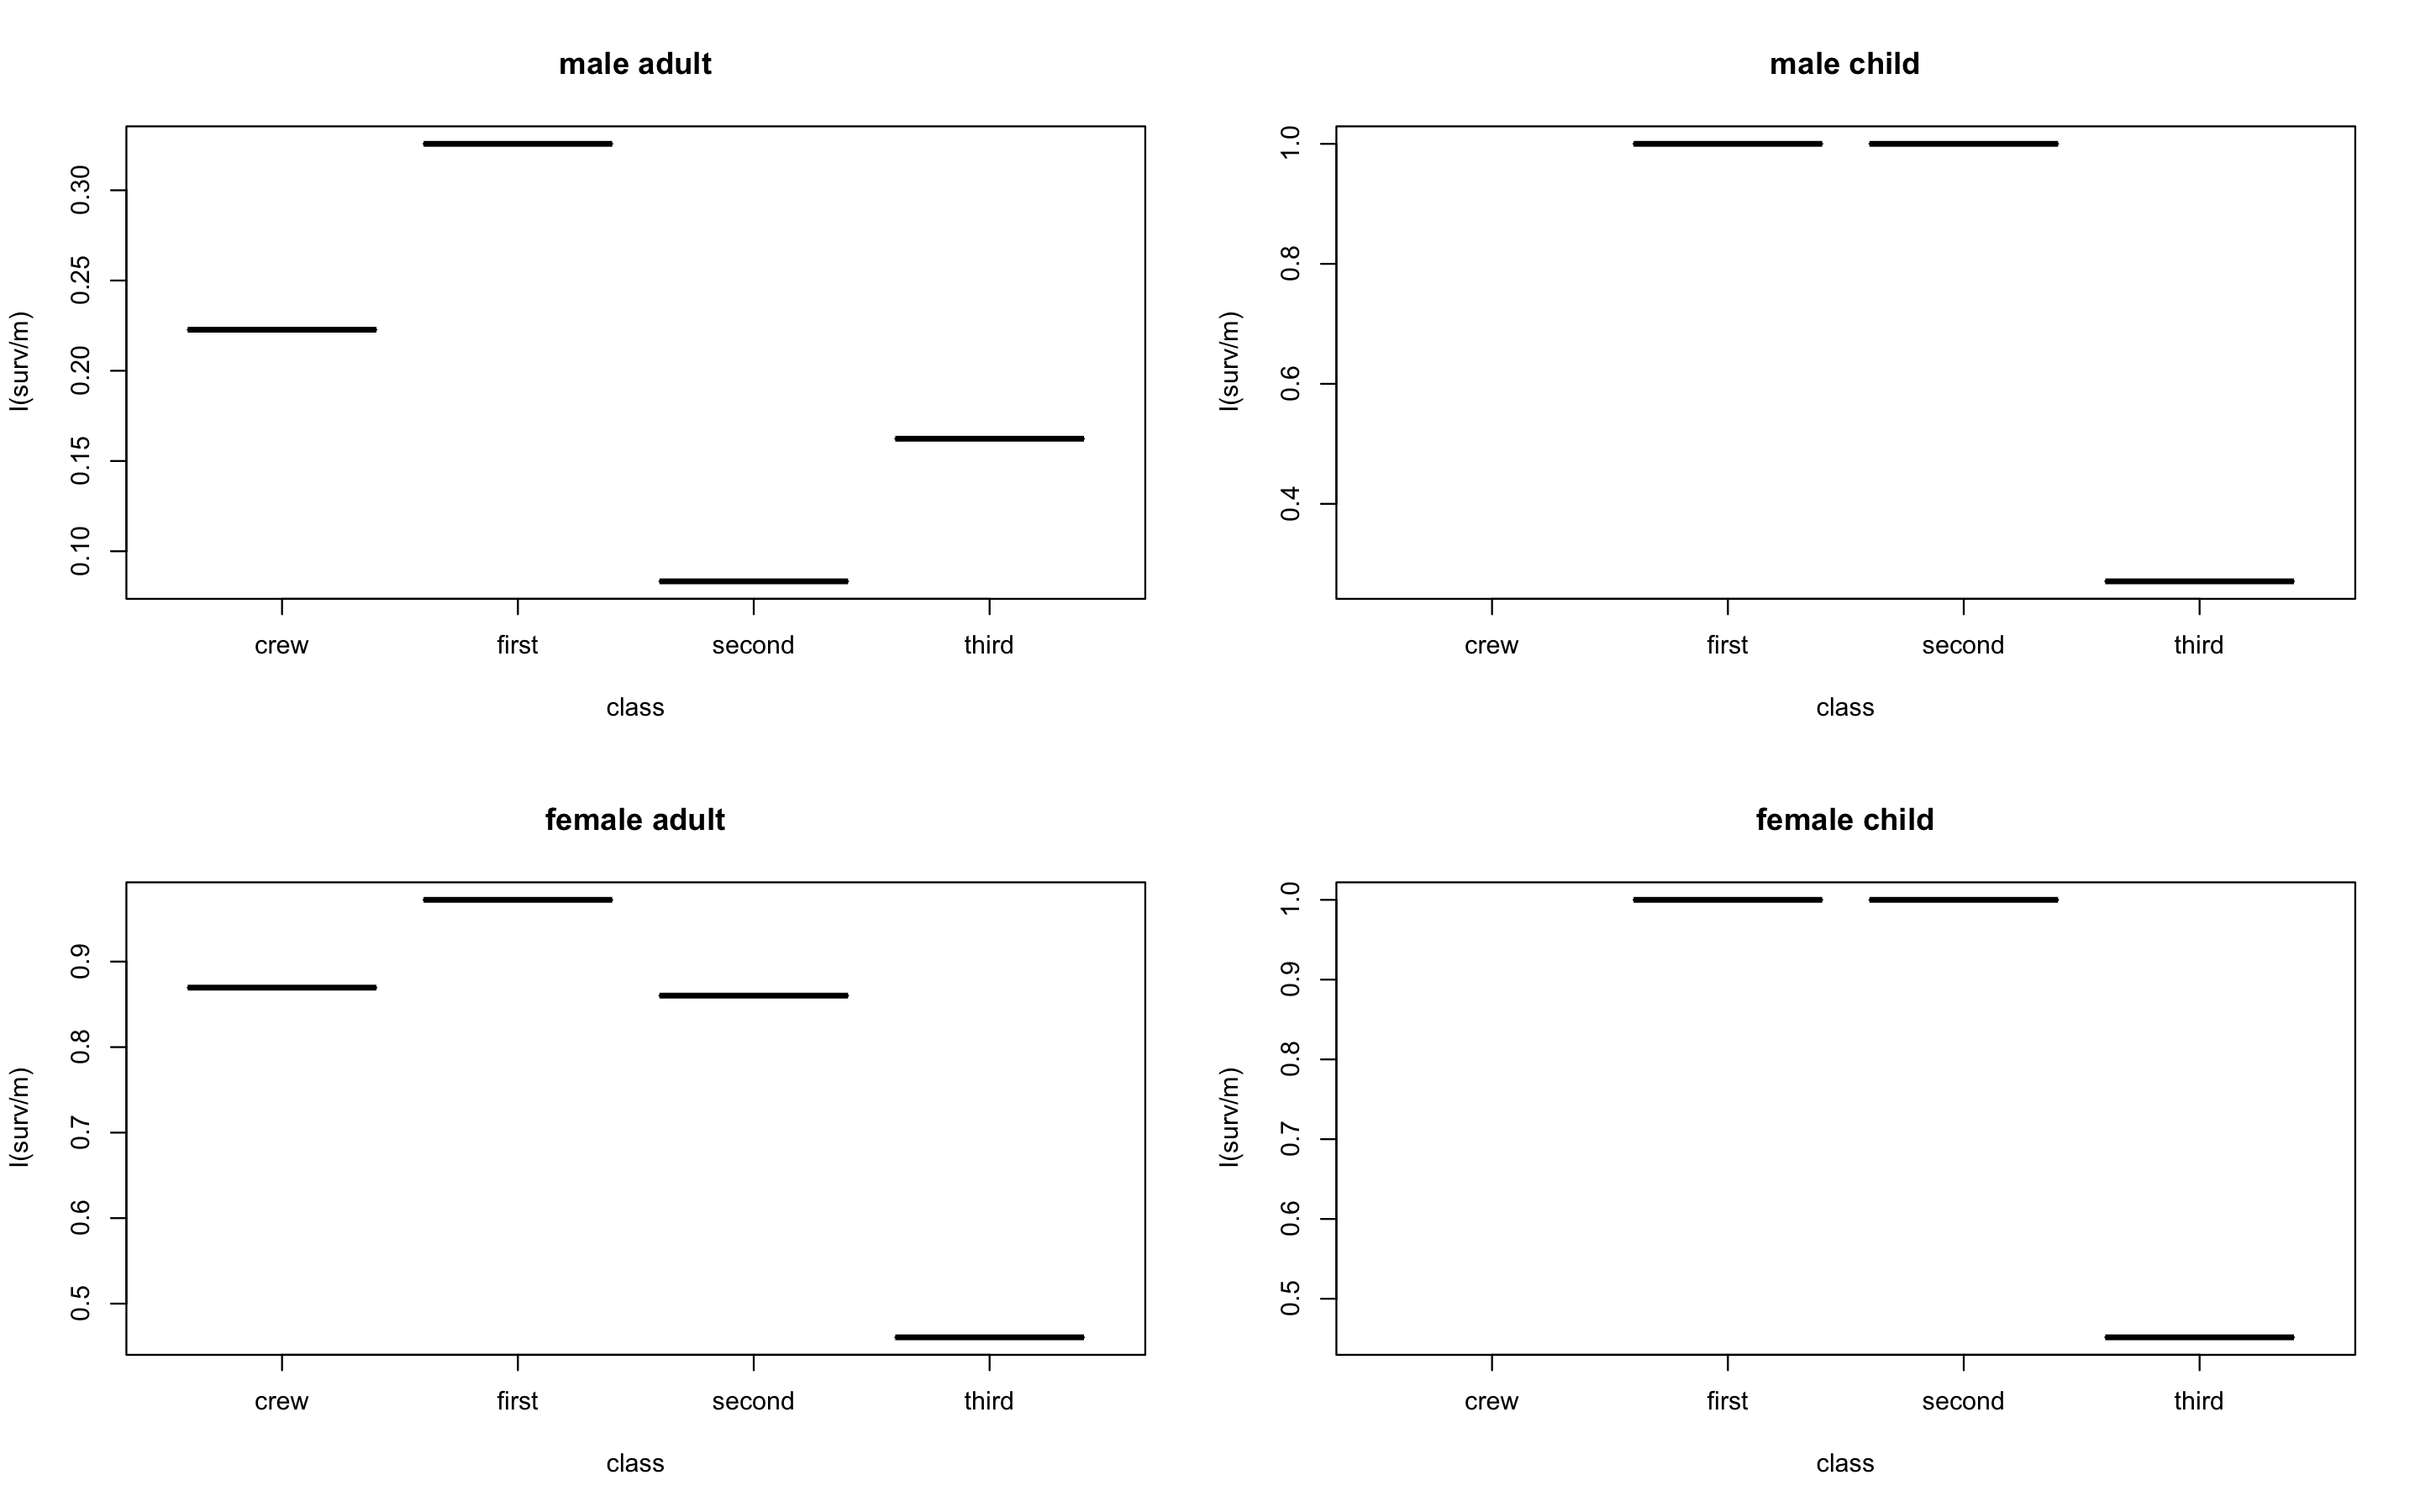
\includegraphics[width=11cm]{Part2_freq1}
	\caption{Prior probabilities of each combination of predictors}
\end{figure}

% Figure 5: priors
\begin{figure}[h]				%placement (here)
	\centering
	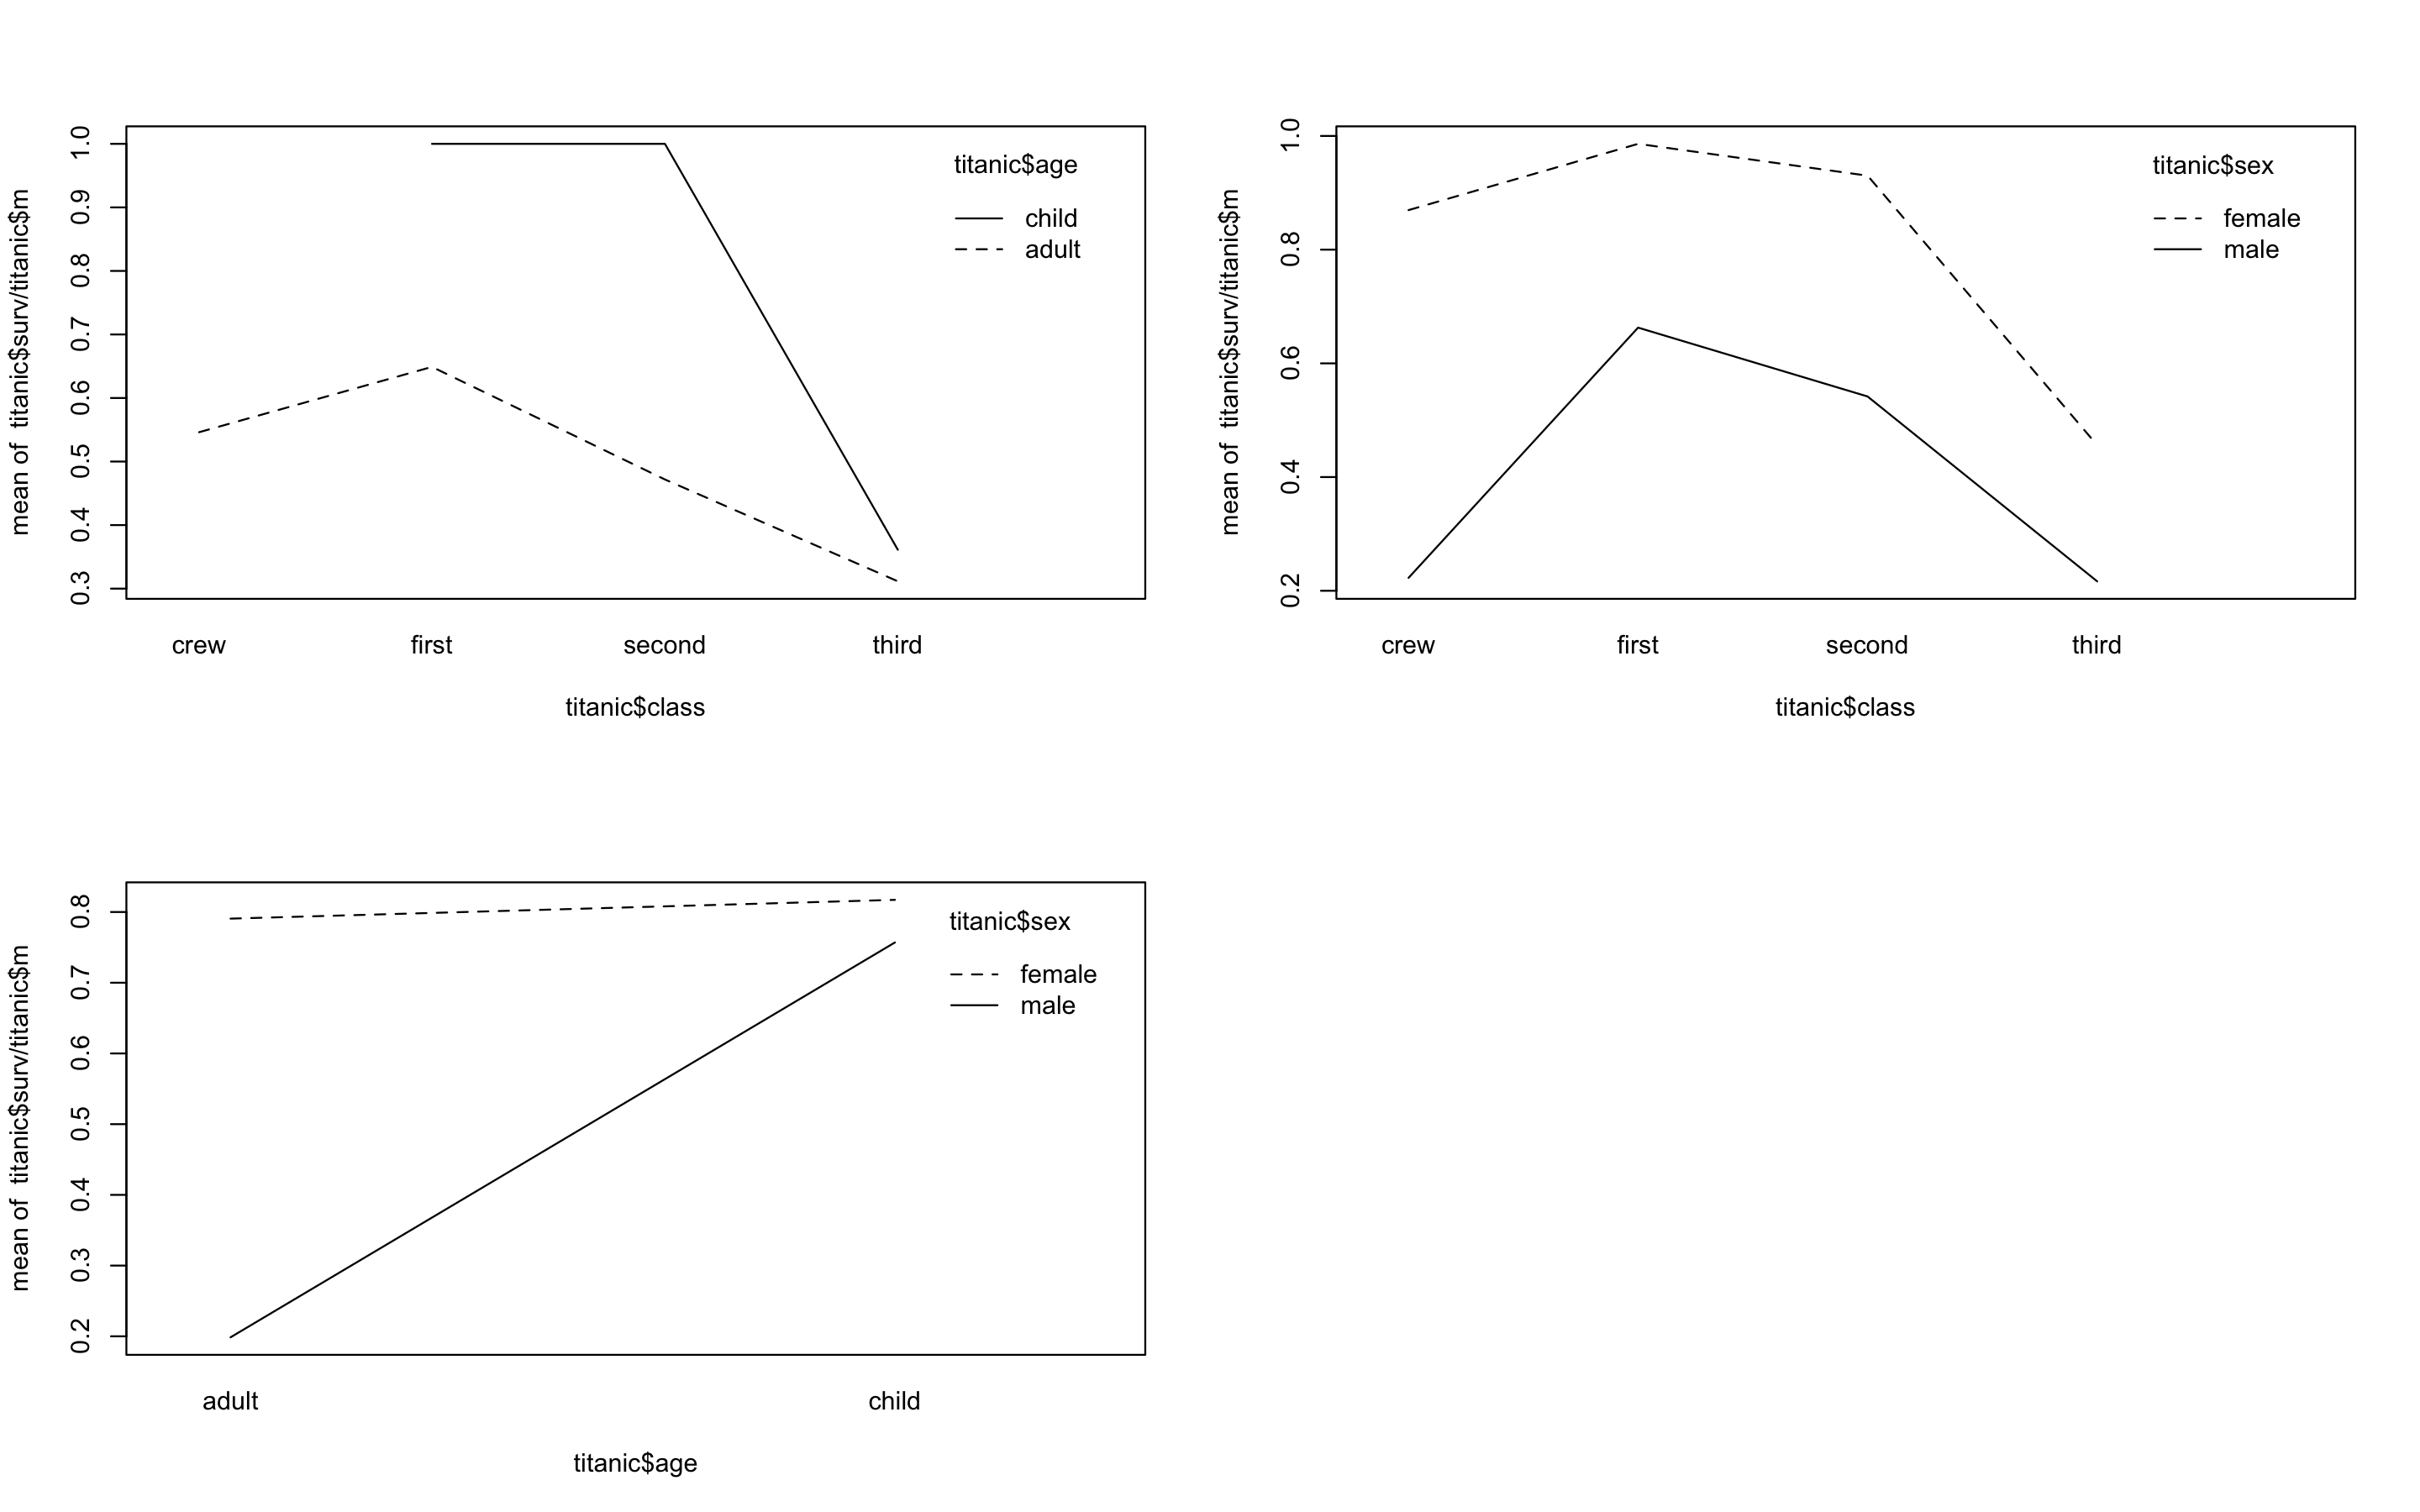
\includegraphics[width=11cm]{Part2_interactions}
	\caption{Interaction plots}
\end{figure}

Figure 5 shows interaction plots of all variables. They clearly show an interaction between class and age, and age and sex variables. This suggests that a model which contains only class, age and sex as predictors is unsuitable for this dataset.

\paragraph{Question 2}
logModel2 is a logistic regression model that contains class, age, sex along with all three two-factor interactions.

% Figure 6: ANOVA
\begin{figure}[h]				%placement (here)
	\centering
	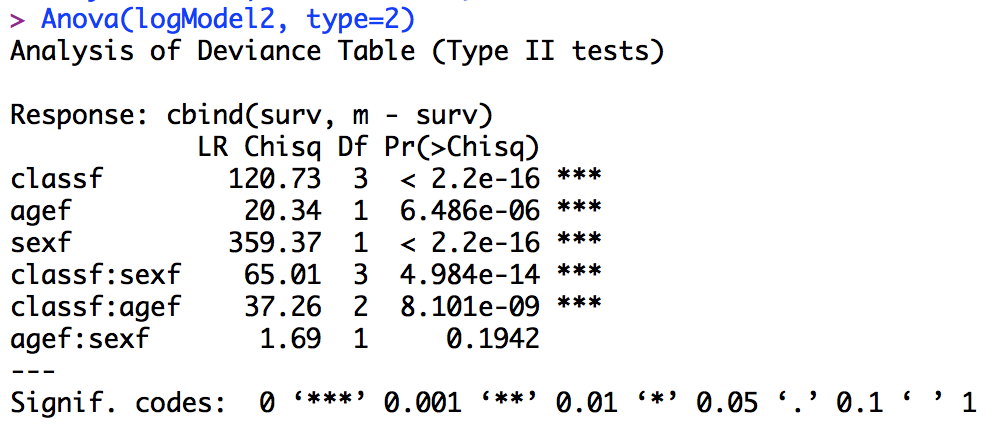
\includegraphics[width=12cm]{Part2_anova}
	\caption{Analysis of Deviance for logModel2}
\end{figure}

\paragraph{}
An ANOVA test on logModel2 shows that removing the age:sex interaction term from the model results in a residual deviance of 1.69, which still indicates a good fit. Dropping class:age produces a residual deviance of 44.2, and dropping class:sex produces a residual deviance of 66.7. This shows that compared to the other interaction terms, age:sex doesn't contribute much to the log-likelihood function of the model. The command used was Anova(logModel2, type=2), which computes a Likelihood Ratio chi-squared test for each addition of a new predictor, respecting the principle of marginality (adding each predictor before any interaction terms it appears in). The p-value of the LR chi-squared test of age:sex was 0.1942, which means we can safely reject the alternative hypothesis (the age:sex coefficient is non-zero) at a threshold of 5\%.

\paragraph{}
A stepwise comparison of the models was performed using the command step(logModel2). The results show that dropping age:sex decreases the AIC of the model from 70.6 to 70.3. This isn't a drastic improvement, but it confirms that this interaction term doesn't improve the model significantly.

The speculation in part 1 about age and sex being correlated may be justified if the variation in the age:sex interaction term was affected by other variables. In this case, the added variable plot of age:sex would be very spread out, indicating that the variation in the response not due to the other predictors is poorly explained by the variation of age:sex not due to other predictors. In other words, including the effect of other predictors on the variation of age:sex might better explain the variation of the response. This is confirmed in figure 7.

% Figure 7: avPlot
\begin{figure}[h]				%placement (here)
	\centering
	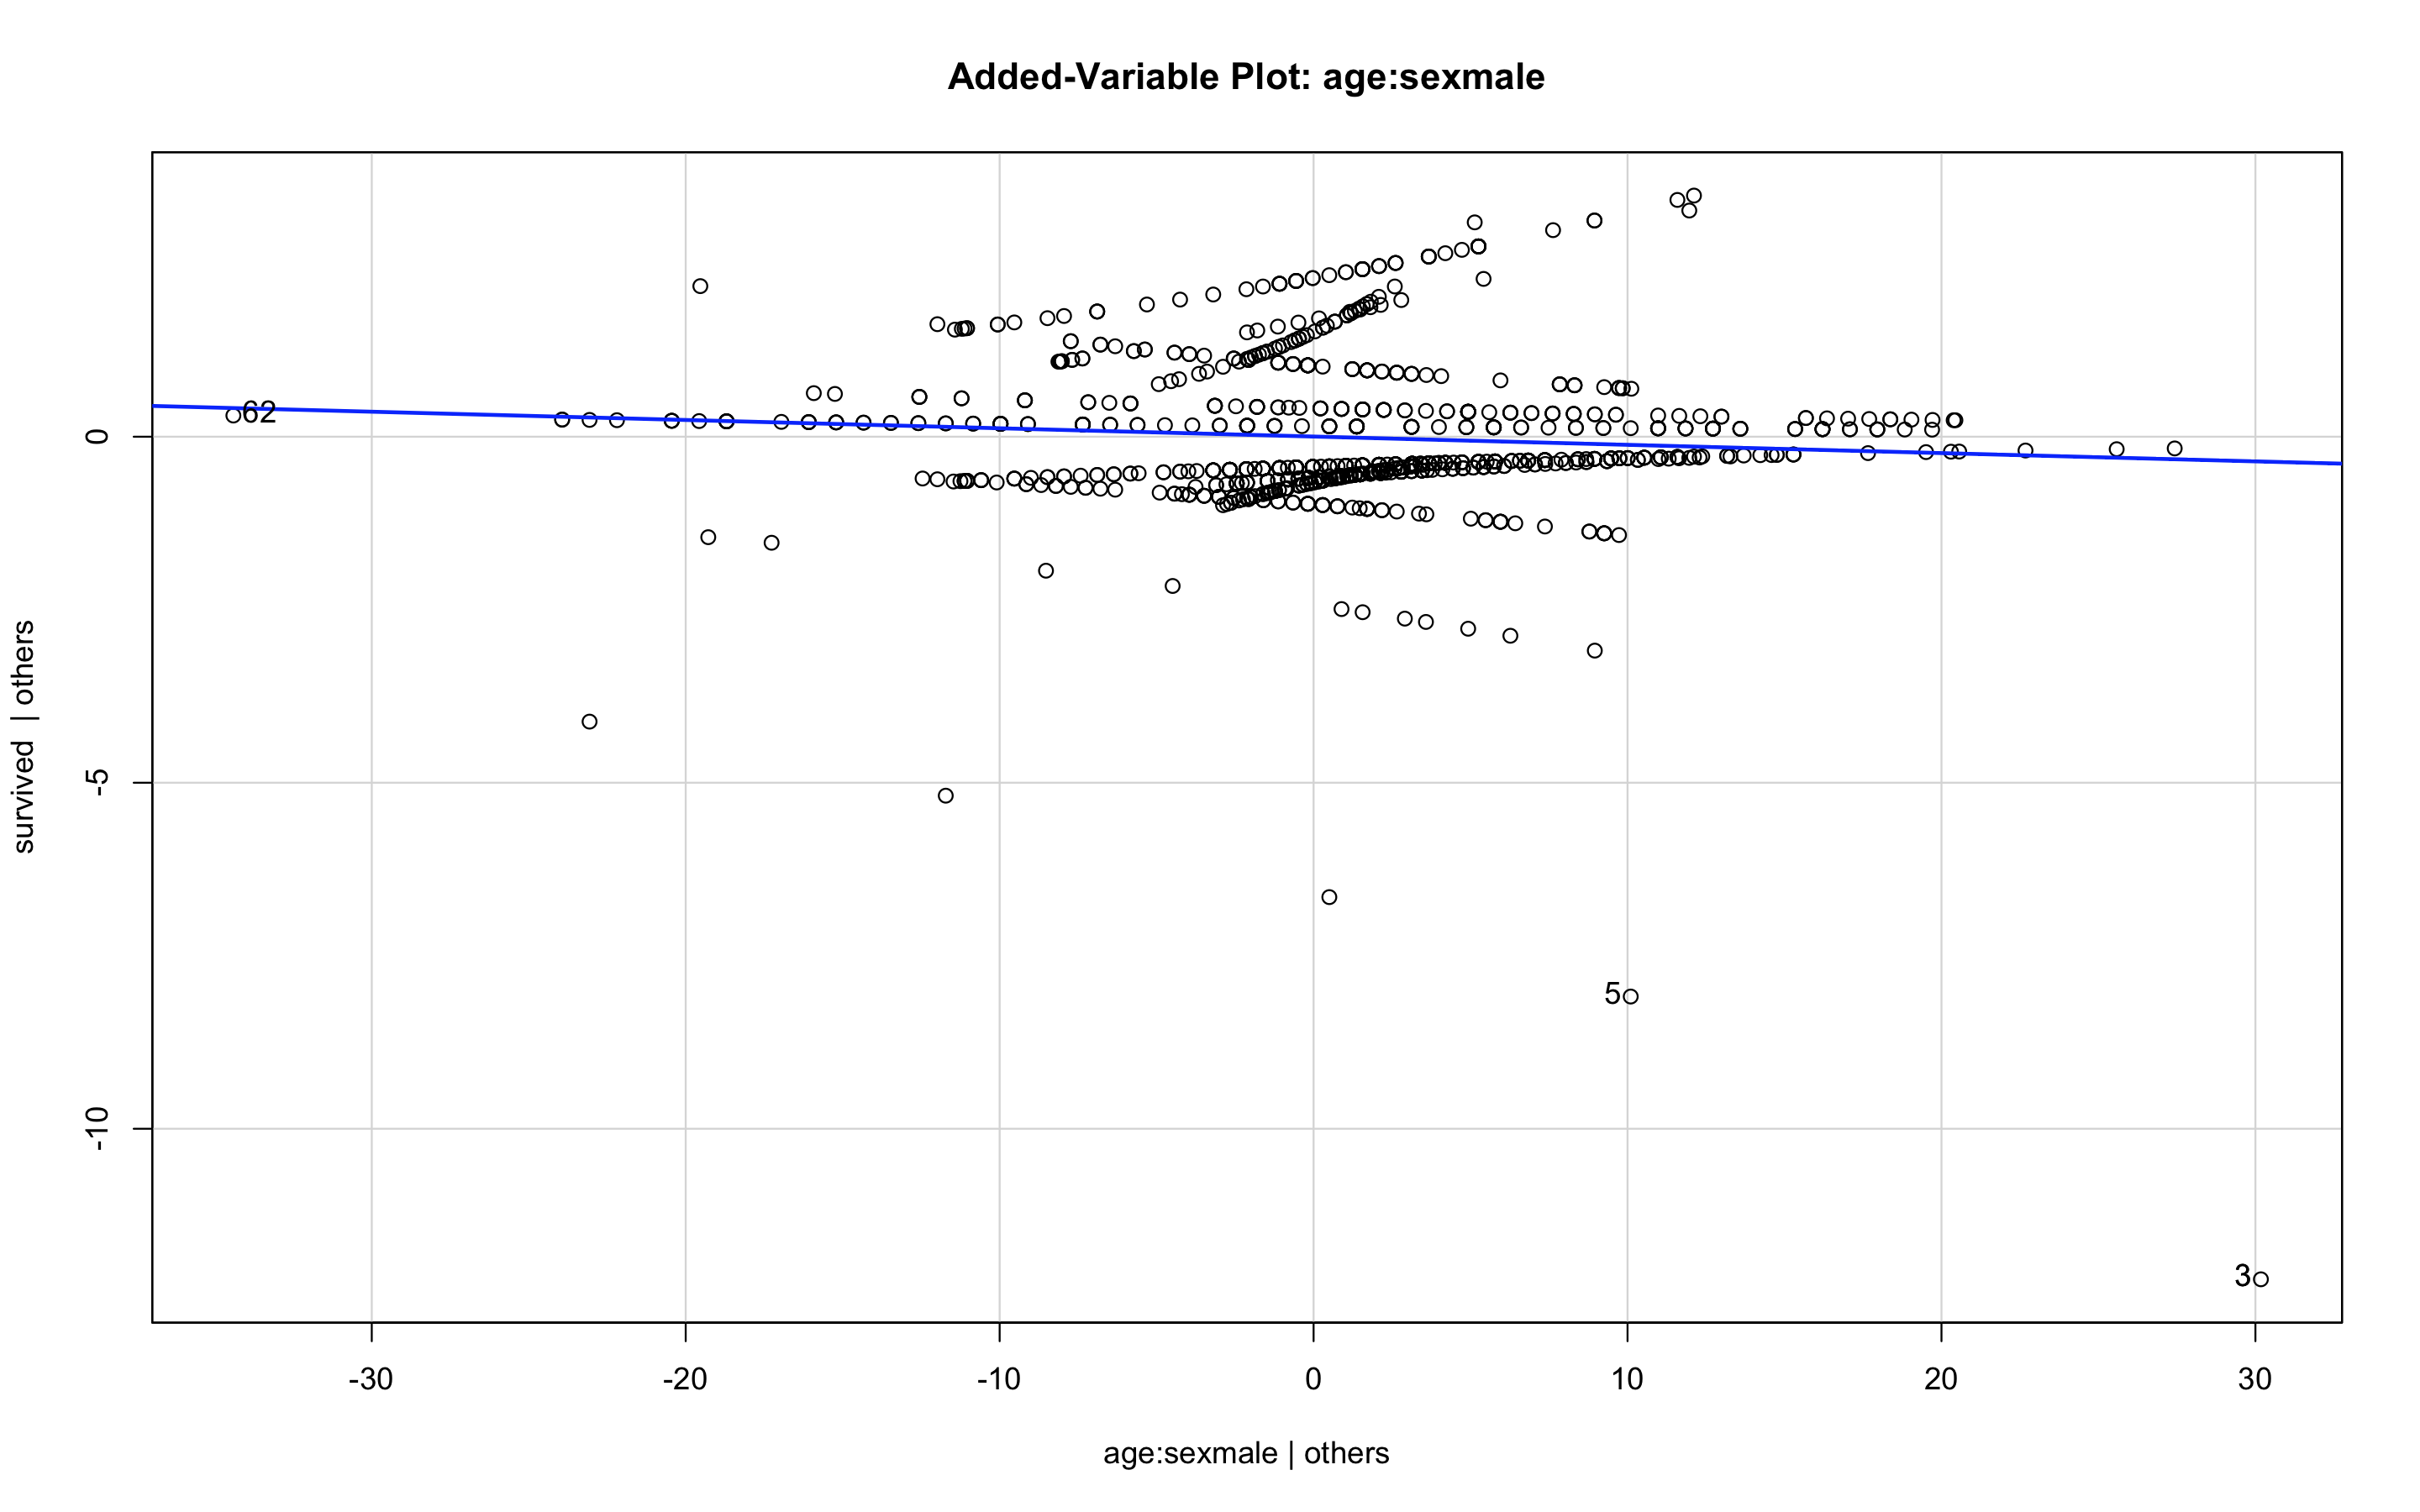
\includegraphics[width=10cm]{Part2_avplot}
	\caption{Added variable plot for age:sex interaction variable}
\end{figure}

% Figure 8: summary
\begin{figure}[h]				%placement (here)
	\centering
	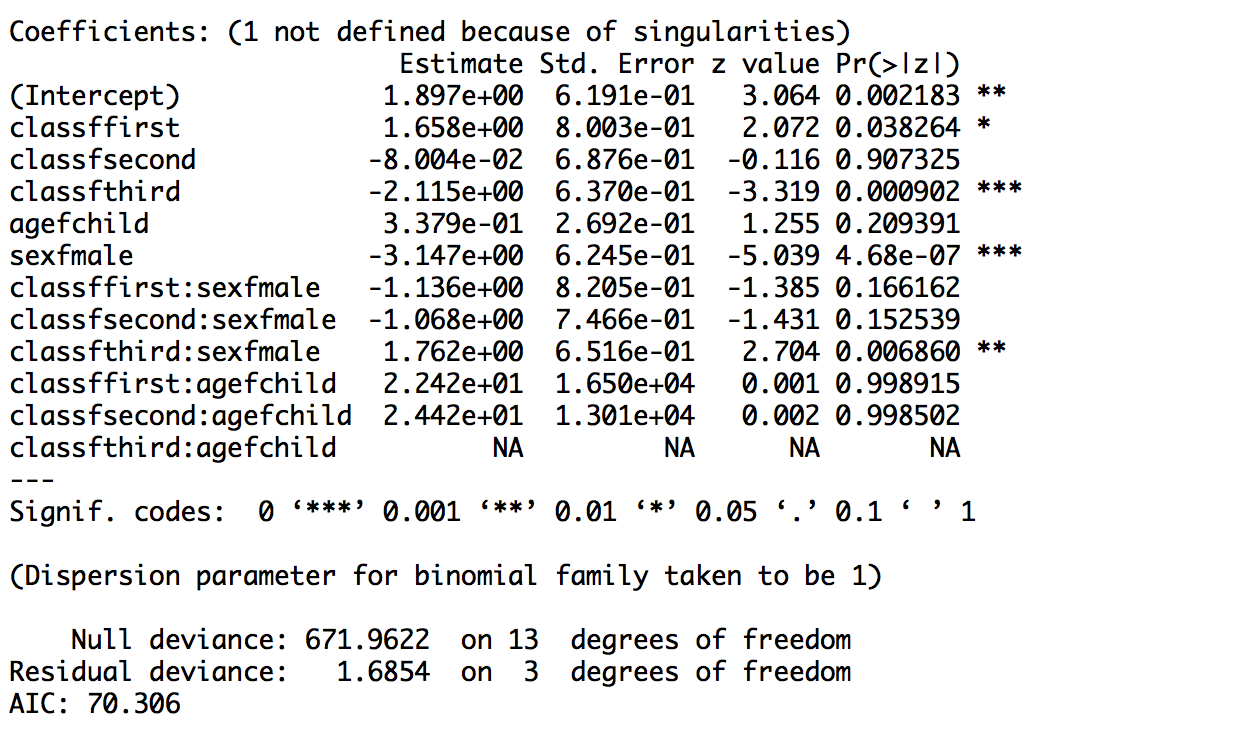
\includegraphics[width=12cm]{Part2_summary}
	\caption{Summary of final model, with only class:age and class:sex interactions}
\end{figure}

\paragraph{}
From the estimates obtained in the final model (figure 8), we see that first class passengers had a log-odds ratio of surviving of 1.658, and those in third class had a log-odds ratio of -2.115. This means that the odds of surviving among first class passengers was 5.25 times that of the other classes, while those of third class were 0.12 times that of the other classes. These odds translate to a 13\% chance of survival for third class, and 84\% chance for first class passengers, knowing that the prior probability of survival for the entire population was 32\%.

\paragraph{}
According to the model, children seem to have been equally likely to survive between first and third classes. The coefficient for the firstclass/child dummy variable has a p-value in excess of 0.99, so does the secondclass/child dummy variable. This is confirmed in an ANOVA test using the ungrouped data: removing the class:age variable from the model results in a deviance of only 0.483. Note that class:age was a meaningful predictor with the ungrouped dataset. This is because in the ungrouped dataset, age is a continuous variable, whereas it was a categorical variable in the grouped dataset. While in both the grouped and ungrouped dataset the coefficients for class:age were close to zero and their p-values were high (0.998 and 0.488 resp.), keeping the interaction between class and age in the grouped dataset yields a better model fit. Looking at the prior probabilities shows clearly that children in third class had a much lower survival rate than the rest, but this pattern isn't captured by the model.



\end {document}